% Degrees of freedom needed for the first 1000 eigenvalues: the largest relative
% error over the block against the degrees of freedom, one curve per
% discretisation, with the tolerances as levels and the extrapolations beyond the
% sweep as dotted continuations. H-shaped domain.
%
% The domain has no closed-form spectrum, so the reference is a DST run of its
% own at M = 161, 19981 degrees of freedom, finer than every run of the sweep.
% Being a computation it carries an error of its own, and the grey line marks it:
% the reference floor, the distance between the reference and the finest DST run
% below it. A tolerance within an order of magnitude of that floor is not
% resolved by this computation, and against a DST reference the DST curve
% measures agreement between two DST runs rather than distance from the exact
% eigenvalues. The FD and FEM curves, whose errors are orders of magnitude
% larger, are unaffected.
%
% H has six re-entrant corners, more than any other domain of the catalogue, and
% each carries the same r^(2/3) singularity as the one of the L-shape. The rates
% the curves settle on are to be read against that.
%
% Requires in the preamble:
%   \usepackage{graphicx}
%   \usepackage{epstopdf}   % the figure is EPS; needed under pdflatex,
%                           % which then wants -shell-escape. Not needed for
%                           % latex/dvips, which reads EPS directly.
%
% The figure lives next to this file, in results/eigenvalues_dof_requirement/.
% If you \input this snippet from elsewhere, point graphicx at that folder, e.g.
%   \graphicspath{{results/eigenvalues_dof_requirement/}}
% and drop the leading path from the \includegraphics argument below.

\begin{figure}[htbp]
  \centering
  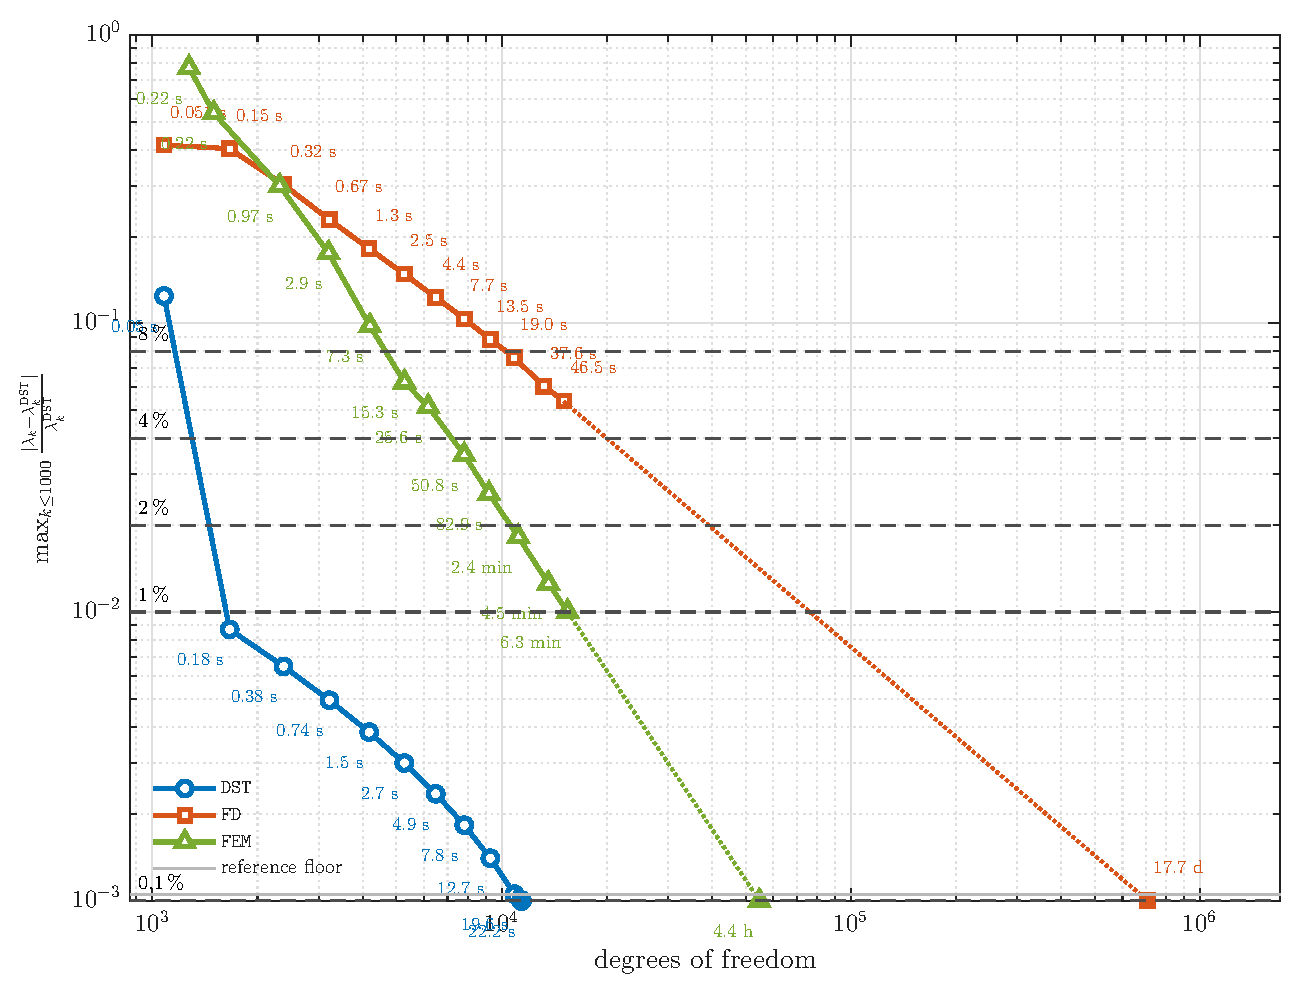
\includegraphics[width=0.85\textwidth]{H_shaped_dof_requirement_n1000}
  \caption{Accuracy of the first 1000 eigenvalues of Laplace operator, zero Dirichlet boundary conditions, H-shaped domain \texttt{H\_shaped}. Largest relative error over the whole block of first $1000$ eigenvalues, $\left\{ \lambda_k \right\}_{k=1}^{1000}$, $\max_{k \leq 1000} \frac{|\lambda_k - \lambda_k^{\text{DST}}|}{\lambda_k^{\text{DST}}}$, against the degrees of freedom used by each discretisation of Laplace operator, compared with the reference eigenvalues computed by \texttt{DST} with 19981 degrees of freedom; \texttt{FEM} -- finite element method, \texttt{FD} -- finite differences method, \texttt{DST} -- discrete sine transform method. Each marker is labelled with the computation time of the particular run, dotted lines show extrapolated values.}
  \label{fig:dof_requirement_H_shaped}
\end{figure}
